% Copyright (c)  2005-2010 EDF-EADS-PHIMECA.
% Permission is granted to copy, distribute and/or modify this document
% under the terms of the GNU Free Documentation License, Version 1.2
% or any later version published by the Free Software Foundation;
% with no Invariant Sections, no Front-Cover Texts, and no Back-Cover
% Texts.  A copy of the license is included in the section entitled "GNU
% Free Documentation License".
\renewcommand{\filename}{docUC_InputNoData_ComposedDistribution.tex}
\renewcommand{\filetitle}{UC : Creation  of nD distribution from (marginals, copula)}

% \HeaderNNIILevel
% \HeaderIILevel
\HeaderIIILevel





\index{Composed Distribution}
\index{Copula!Independent}
\index{Copula!Normal}
\index{Correlation!Correlation matrix of the Normal copula}
\index{Correlation!Spearman rank correlation matrix}
\index{Distribution!Marginals and copula}


The objective of the Use Case is to model a distribution, described by its marginal distributions and its dependence structure (a particular copula). A simplified way is proposed when the copula is the independent one.\\

Details on copula may be found in the Reference Guide (\href{OpenTURNS_ReferenceGuide.pdf}{see file Reference Guide - Step B -- Copula}).\\

Details on each object may be found in the User Manual  (\href{OpenTURNS_UserManual_TUI.pdf}{see User Manual - Probabilistic modeling / Composed Distributions}).\\

This Use Case is particularly adapted to the modelisation of the distribution of the input random vector.\\

The example here is a distribution of dimension 3 defined by :
\begin{itemize}
\item Beta, Triangular and Uniform marginals,
\item an independent copula.
\end{itemize}

\noindent%
\requirements{
  \begin{description}
  \item[$\bullet$] none
  \end{description}
}
{
  \begin{description}
  \item[$\bullet$] a nD distribution : {\itshape myDistribution}
  \item[type:] Distribution which implementation is a ComposedDistribution
  \end{description}
}

\textspace\\
Python script for this UseCase :

\begin{lstlisting}

  # Create the first marginal : Weibul(mu, sigma, gamma) = Weibull(2.0, 1.0, 0.0)
  weibDist = Weibull(2.0, 1.0, 0.0, Weibull.MUSIGMA)
  weibDist.setName("First Marginal : Weibull")

  # Create the second marginal : Triangular(a,m,b) = Triangular(1.0, 3.0, 5.0)
  triangularDist = Triangular(1.0, 3.0, 5.0)
  triangularDist.setName("Second Marginal : Triangular")

  # Create the third marginal : Uniform(a,b) = Uniform(2.0, 4.0)
  uniformDist = Uniform(2.0, 4.0)
  uniformDist.setName("Third Marginal : Uniform")


  # Create a collection of distribution of dimension 3
  # using List python
  aCollection = DistributionCollection([weibDist, triangularDist, uniformDist])
  
  # Create a copula : Normal copula of dimension 3 fom Spearman rank correlation matrix
  spearmanMatrix = CorrelationMatrix(3)
  spearmanMatrix[0,1] = 0.25
  spearmanMatrix[1,2] = 0.25
  aCopula = NormalCopula(NormalCopula.GetCorrelationFromSpearmanCorrelation(spearmanMatrix))
  aCopula.setName("Normal copula")


  # CASE 1 : not independent copula

  # Instanciate one distribution object
  myDistribution = ComposedDistribution(aCollection, aCopula)

  # Give a Description to the Distribution
  myDistribution.setDescription( ( "X1 distribution", "X2 distribution", "X3 distribution", ) )

  # CASE 2 : independent copula

  # It is not necessary to specify the copula

  # Instanciate one distribution object :
  myDistribution = ComposedDistribution(aCollection)

\end{lstlisting}
\textspace\\
We draw in Figures \ref{Marginal12} to \ref{Marginal23} the iso-curves of each 2D distribution defined by two of the three components of the distribution.


\begin{figure}[H]
  \begin{center}
    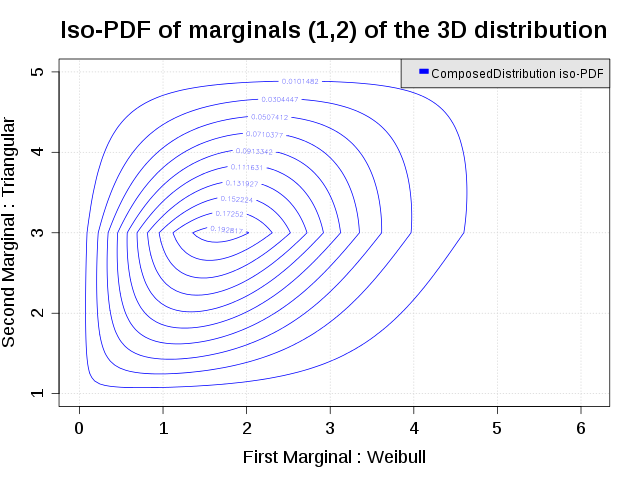
\includegraphics[width=10cm]{ComposedDistribution_isoPDF_12.png}
  \end{center}
  \caption{Iso-PDF of the distribution defined by the marginals 1 and 2.}
  \label{Marginal12}
\end{figure}

\begin{figure}[H]
  \begin{center}
    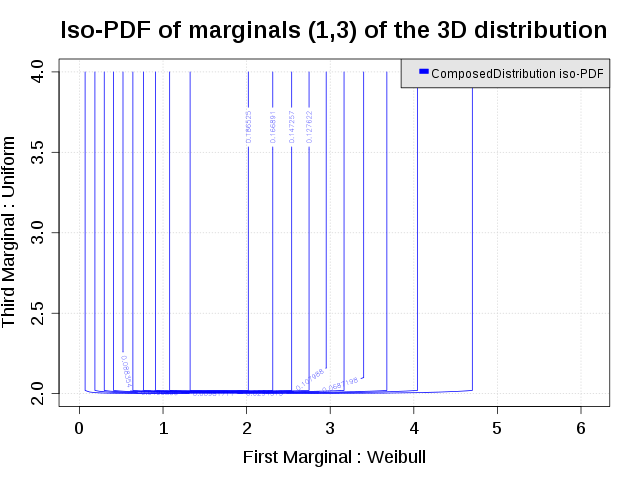
\includegraphics[width=10cm]{ComposedDistribution_isoPDF_13.png}
  \end{center}
  \caption{Iso-PDF of the distribution defined by the marginals 1 and 3.}
  \label{Marginal13}
\end{figure}

\begin{figure}[H]
  \begin{center}
    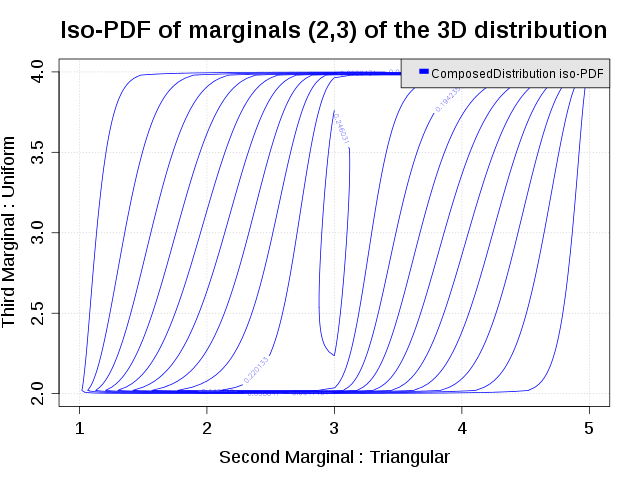
\includegraphics[width=7cm]{ComposedDistribution_isoPDF_23.png}
  \end{center}
  \caption{Iso-PDF of the distribution defined by the marginals 2 and 3.}
  \label{Marginal23}
\end{figure}


